\documentclass{article}

\usepackage{arxiv}

\usepackage[utf8]{inputenc} % allow utf-8 input
\usepackage[T1]{fontenc}    % use 8-bit T1 fonts
\usepackage{hyperref}       % hyperlinks
\usepackage{url}            % simple URL typesettingf
\usepackage{booktabs}       % professional-quality tables
\usepackage{amsfonts}       % blackboard math symbols
\usepackage{nicefrac}       % compact symbols for 1/2, etc.
\usepackage{microtype}      % microtypography
\usepackage{lipsum}
\usepackage{graphicx}
\usepackage{tabularx}
\usepackage{wrapfig}

\usepackage[export]{adjustbox}

\usepackage{xcolor}         % http://ctan.org/pkg/xcolor

\hypersetup{
  colorlinks=true,
  linkcolor=blue!50!red,
  urlcolor=green!70!black
}

\title{An open-source max14866 development board}

\author{
  Luc Jonveaux\thanks{More on the website \url{http://un0rick.cc}. This paper has its on Zenodo DOI  \href{http://doi.org/10.5281/zenodo.5792252}{10.5281/zenodo.5792252} } \\
  Tinkerer, Milly le Meugon, France\\
  \texttt{contact@un0rick.cc} \\
}

%% Wrapping https://tex.stackexchange.com/questions/55161/how-to-arrange-image-and-text-to-appear-side-by-side

\begin{document}
\maketitle

\begin{abstract}
Non destructive testing and imaging ultrasound have been around since the ’50s. Many ultrasound open-source projects are emerging, mostly focusing on image processing - while hardware has been left behind. Several teams have produced successful designs to be used on commercial US scanners, but they are not cheap, and are difficult to access. 

I couldn’t find designs to play with, that would be affordable or open, so I decided to update the previous one, the un0rick, for a more cost-efficient board designed for makers, researchers and hackers.

Having a single-channel device was not enough to play with small linear or annular arrays, so we developped a small high voltage switch control to allow pulse-echo, separating transmit and receive paths, on a 8-element array, or to access up to 16 elements with the same TX/RX path. 

\emph{ This PDF is also a ZIP that contains the sources to the hardware and some data too, don't hesitate to have a look. Just rename the file from .PDF to .ZIP and you're ready to go }.
\end{abstract}

\keywords{open-source \and ultrasound \and hardware \and ice40 \and fpga  }



%                .-') _  .-') _   _  .-')               
%               ( OO ) )(  OO) ) ( \( -O )              
%    ,-.-') ,--./ ,--,' /     '._ ,------.  .-'),-----. 
%    |  |OO)|   \ |  |\ |'--...__)|   /`. '( OO'  .-.  '
%    |  |  \|    \|  | )'--.  .--'|  /  | |/   |  | |  |
%    |  |(_/|  .     |/    |  |   |  |_.' |\_) |  |\|  |
%   ,|  |_.'|  |\    |     |  |   |  .  '.'  \ |  | |  |
%  (_|  |   |  | \   |     |  |   |  |\  \    `'  '-'  '
%    `--'   `--'  `--'     `--'   `--' '--'     `-----' 


\section{Overview}

This wonderful board has been designed to provide a curious tinkerer with the basis to play with, and understand, imaging with multi-element ultrasound sensors.

As stated by its datasheet, "the MAX14866 is a 16-channel, high-voltage (HV), analog SPST switch primarily intended for HV multiplexing in ultrasound applications. The MAX14866 operates from one only low-voltage supply (+5V) and does not require dedicated HV supplies, resulting in cost-saving and system simplification. ". The MAX14866 can transmit undistorted analog signals up to 210VP-P. There are also bleed resistors.

\begin{figure}[htp!]
  \centering
  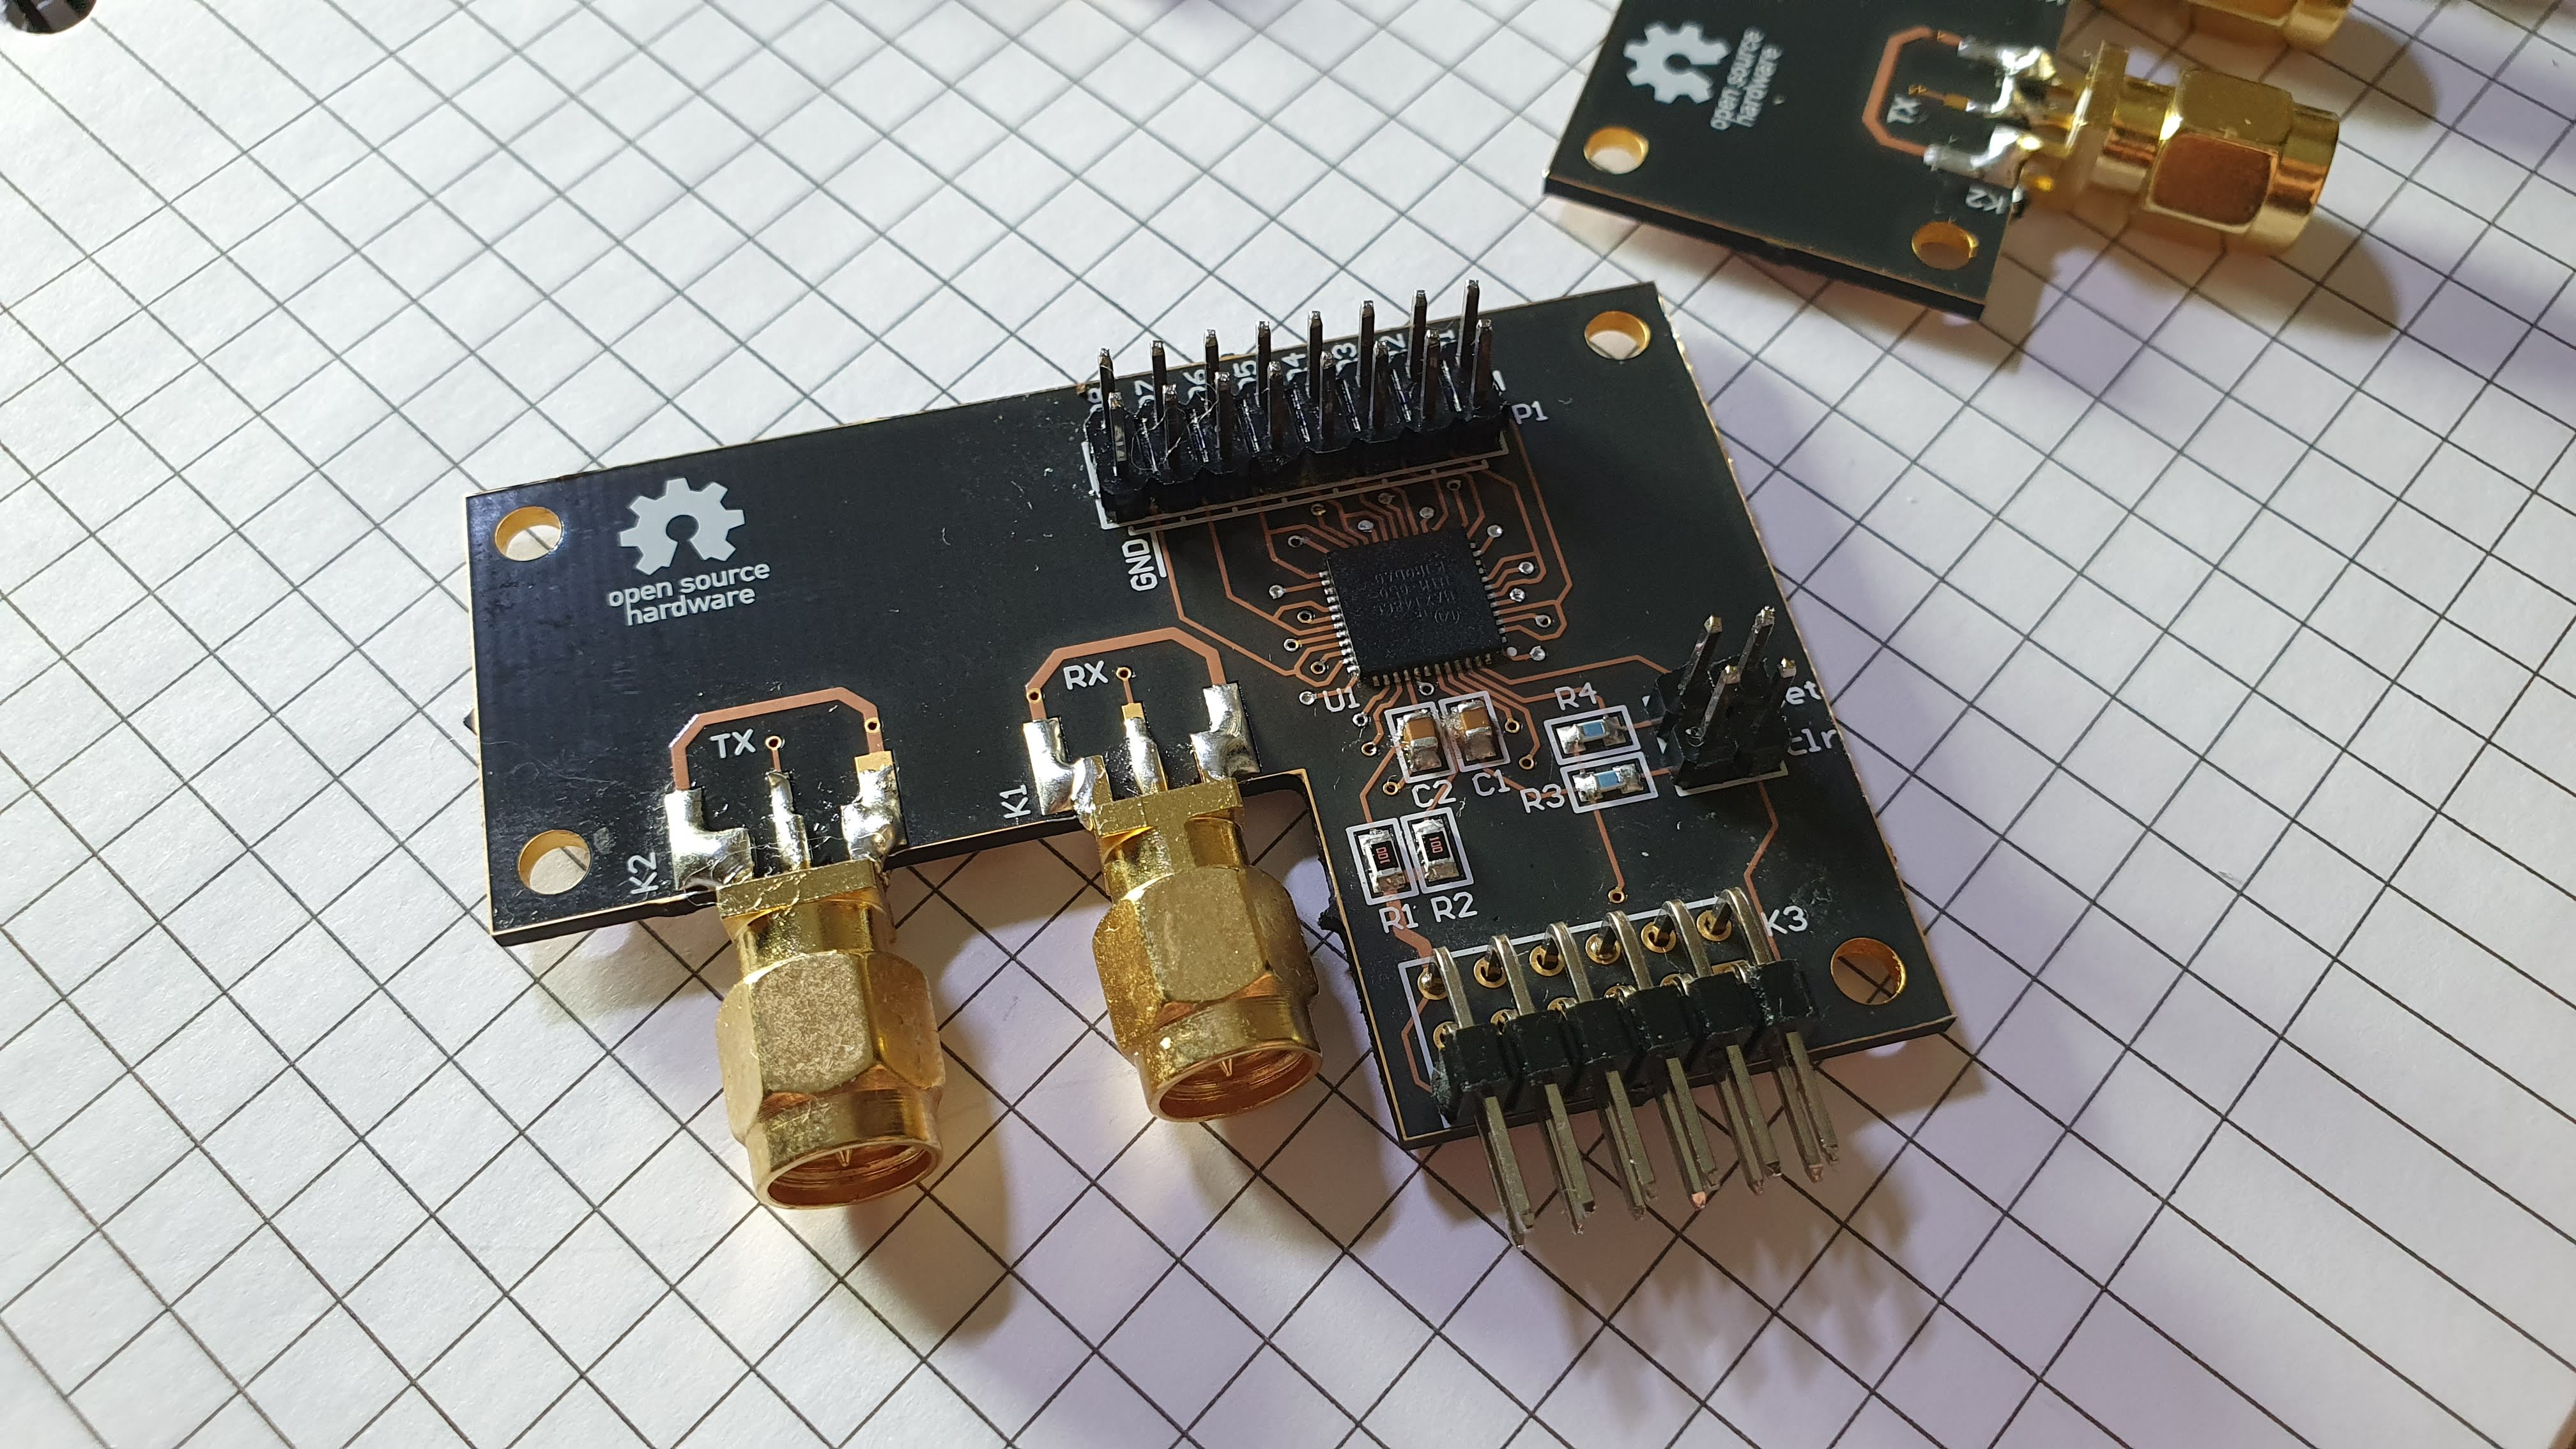
\includegraphics[width=.5\textwidth]{../src/images/20210323_210151.jpg}\hfill
  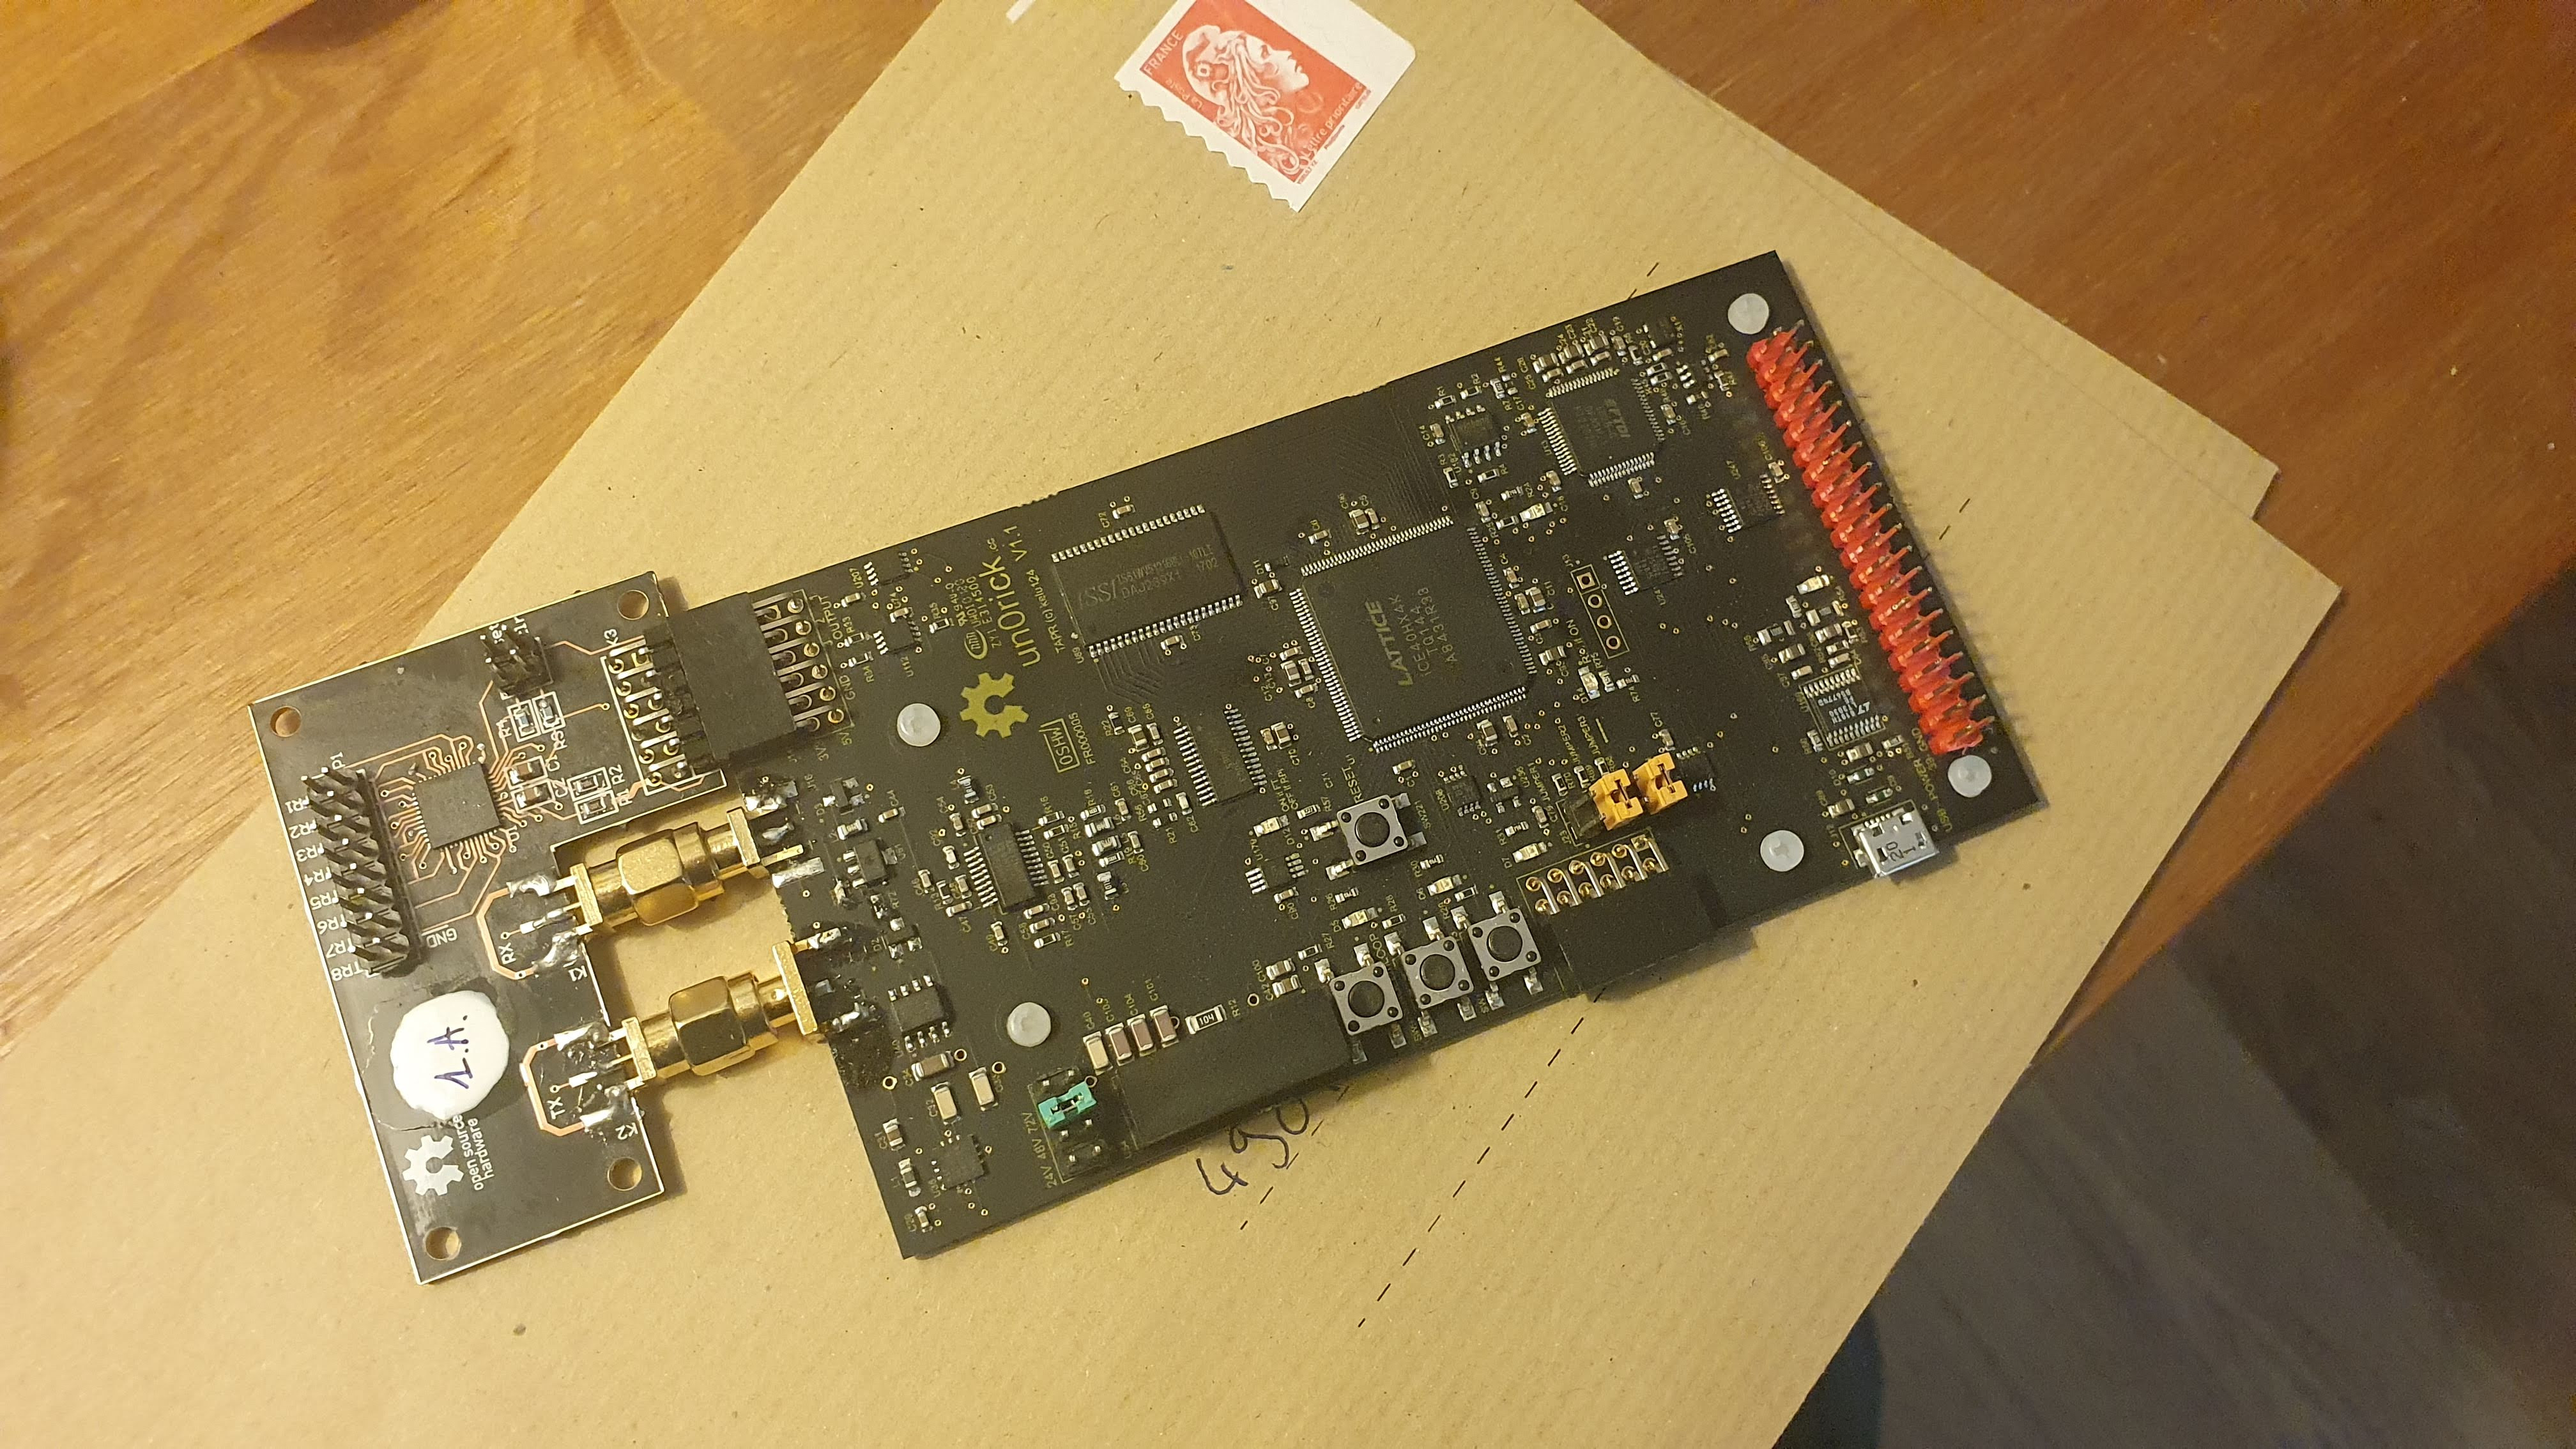
\includegraphics[width=.5\textwidth]{../src/images/20210329_122144.jpg} 
  \caption{Top side of the max14866 board and its connexion to the un0rick.} 
  \label{fig:desc}
\end{figure}
  
This allows for a relatively simple design.


\section{Where to find the latest sources} 
 

The latest sources of the hardware as well as software are available at \url{https://github.com/kelu124/max14866/}. However, this PDF also doubles as an archive (you can rename the .pdf as a .zip, and you'll see), and contains, in short: a set of gerbers and BOM, and some documentation. There may be some other stuff there, but I forgot what I put there.

\section{Operation} 

We have run tests as showed in figure \ref{fig:schme}. The FPGA had all the right logic in place to provide you with a full control over the pulse-echo process.


\begin{figure}[htp!]
  \centering
  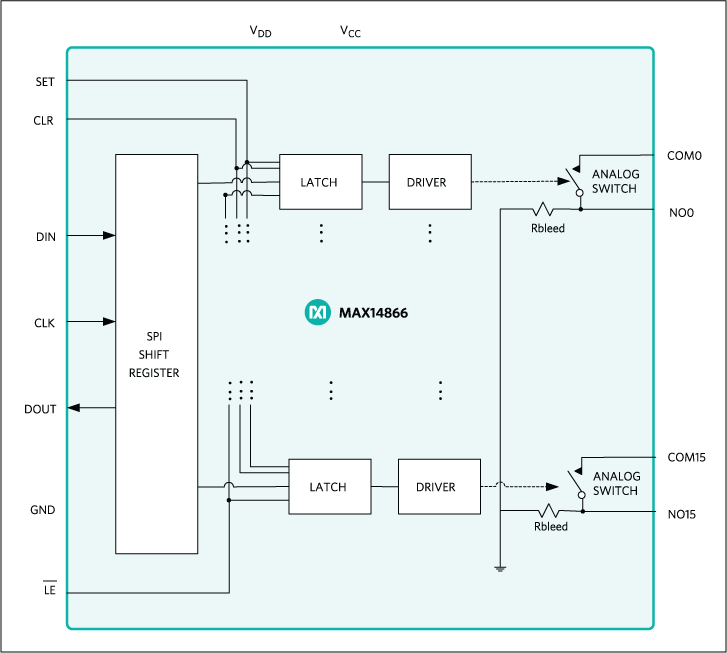
\includegraphics[width=.5\textwidth]{images/9408.png}\hfill
  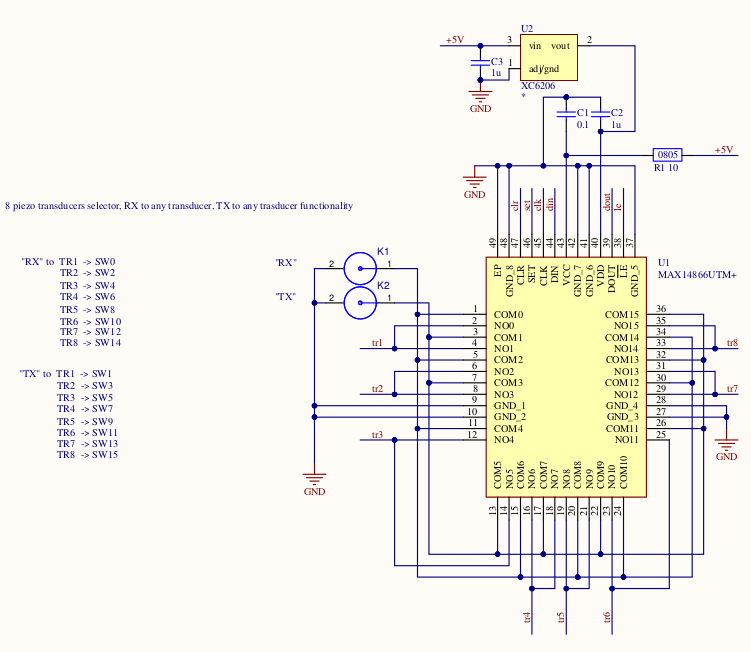
\includegraphics[width=.5\textwidth]{images/schem.png} 
  \caption{Principles of the board} 
  \label{fig:schme}
\end{figure}

The second figure \ref{fig:acq} shows all acquisitions for all pairs of tx/rx combination : we ran the tests on a 5-element arrays, with a pin missed during soldering. That being said, it demonstrates the feasibility to get echoes using the max14866 board.

\begin{figure}[htp!]
  \centering
  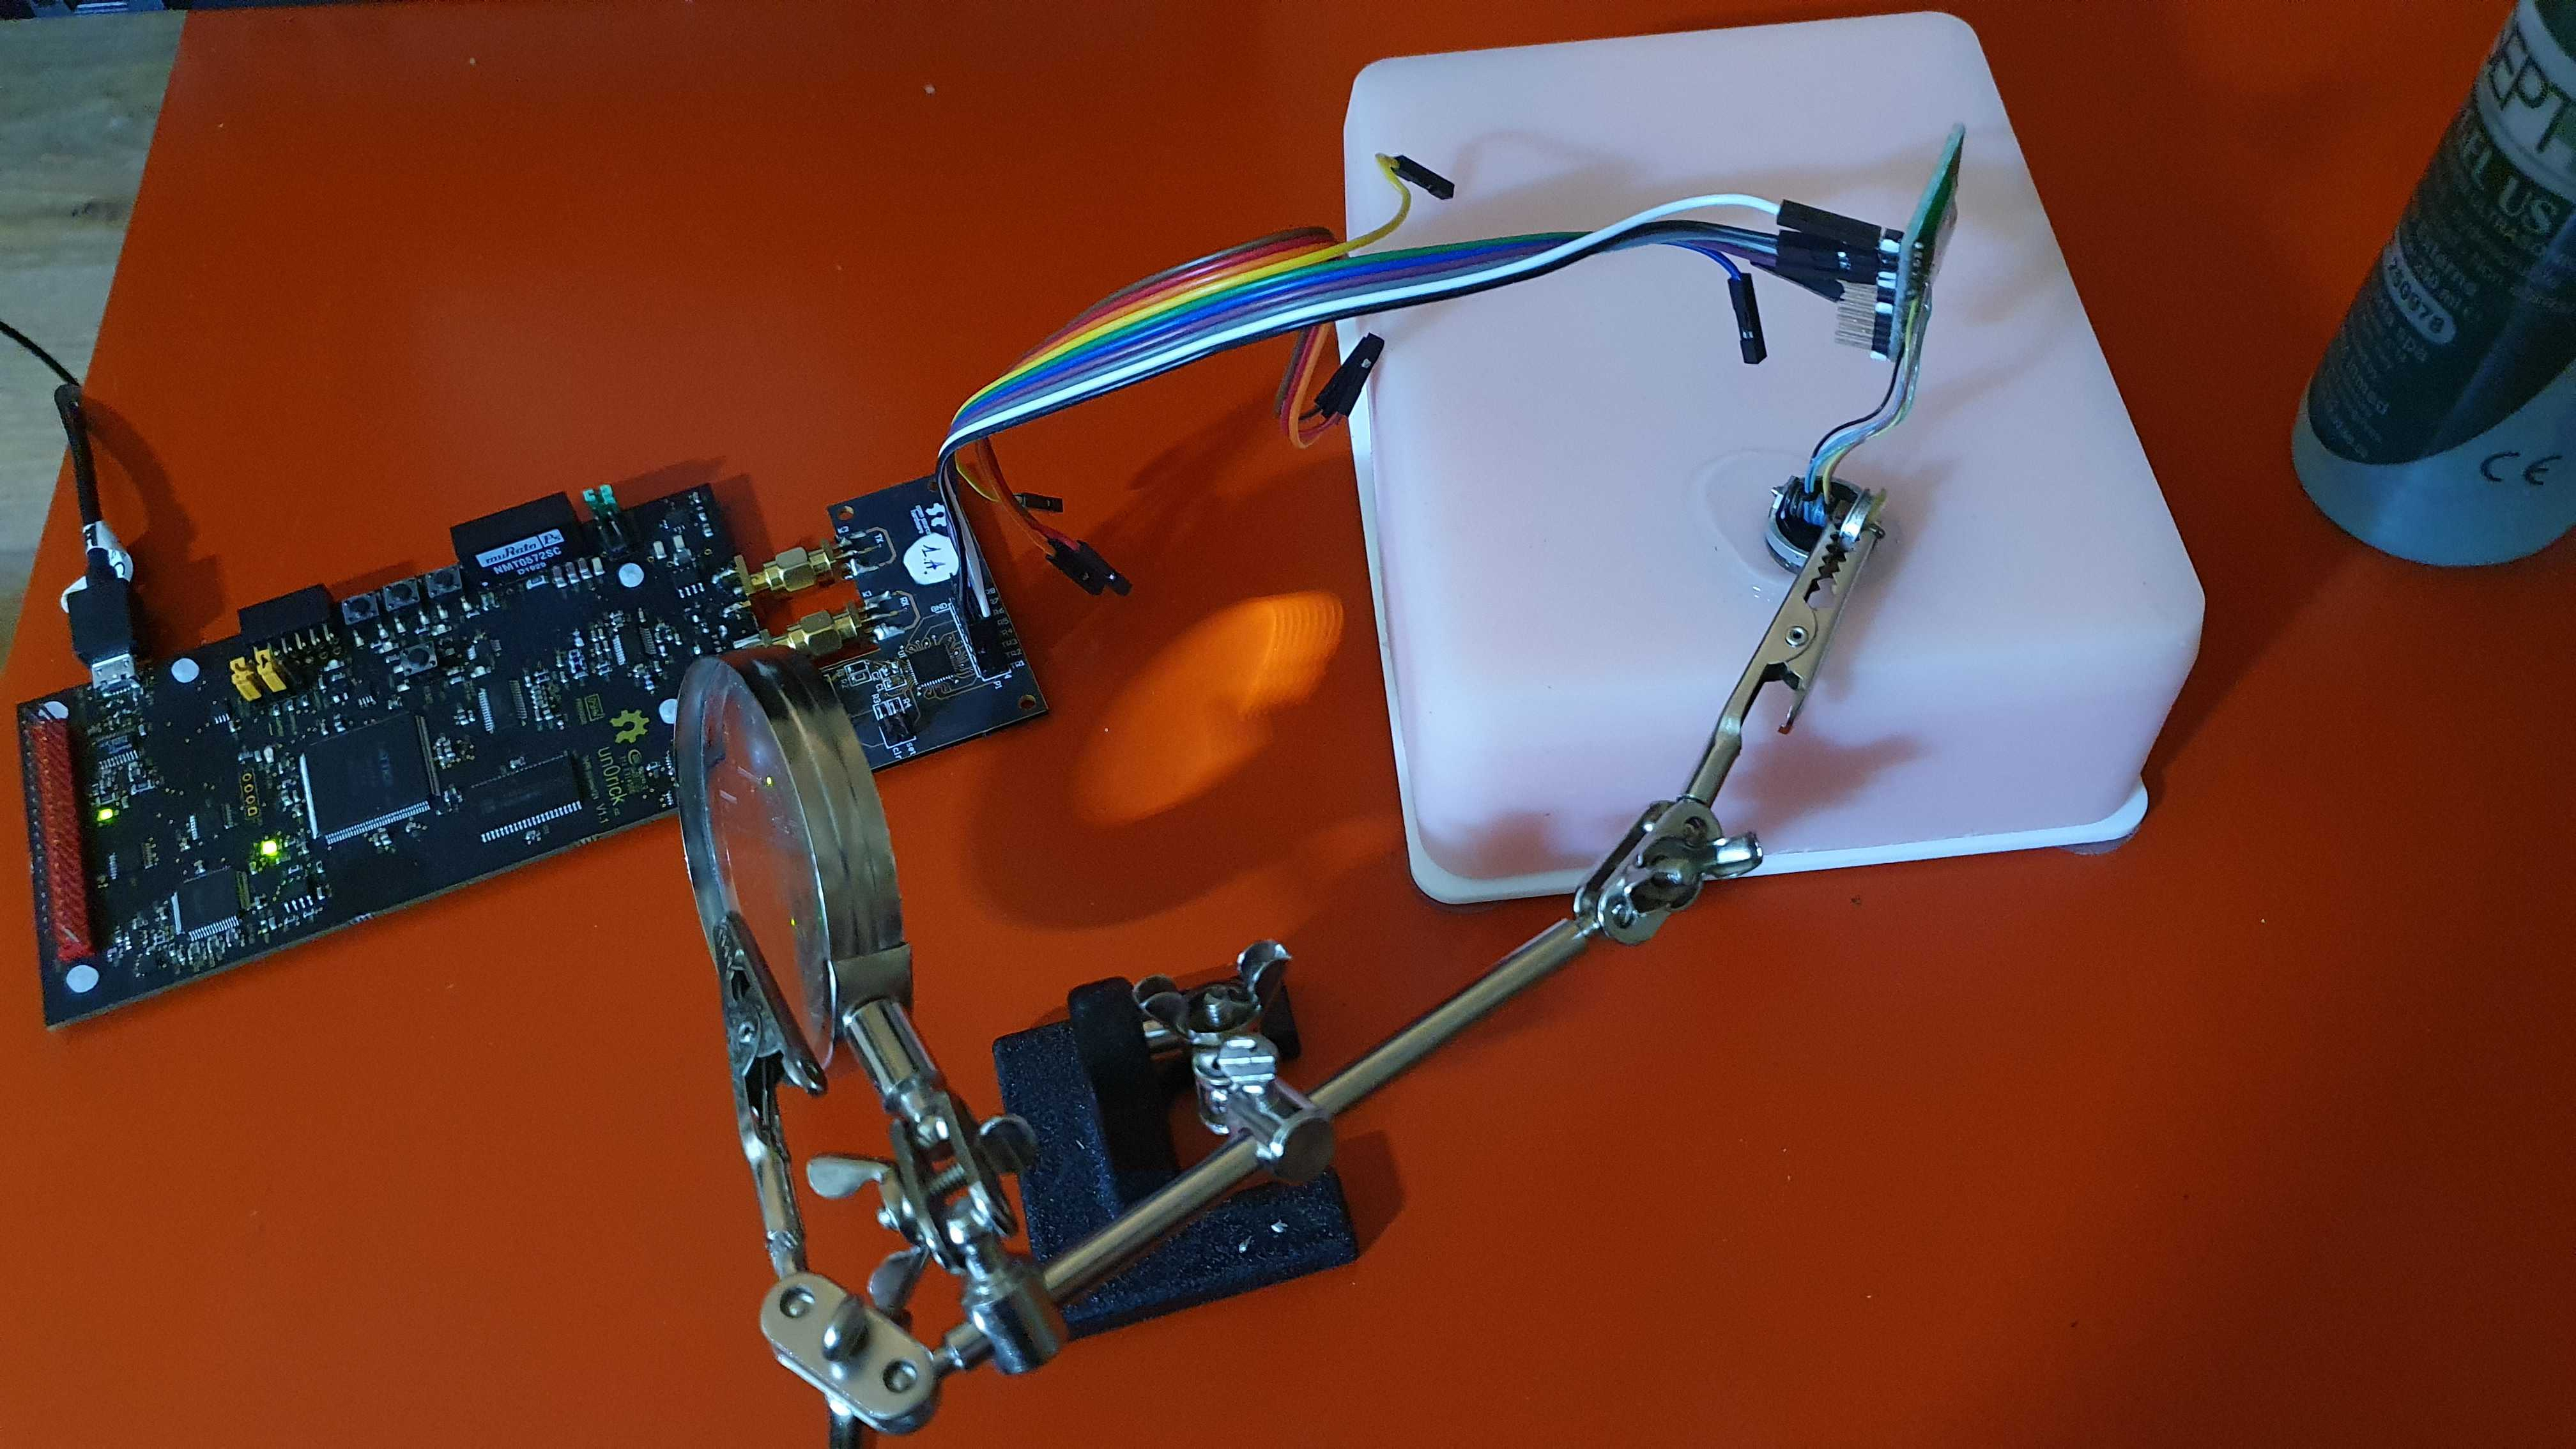
\includegraphics[width=.5\textwidth]{../src/experiment/20210425_203655.jpg}\hfill
  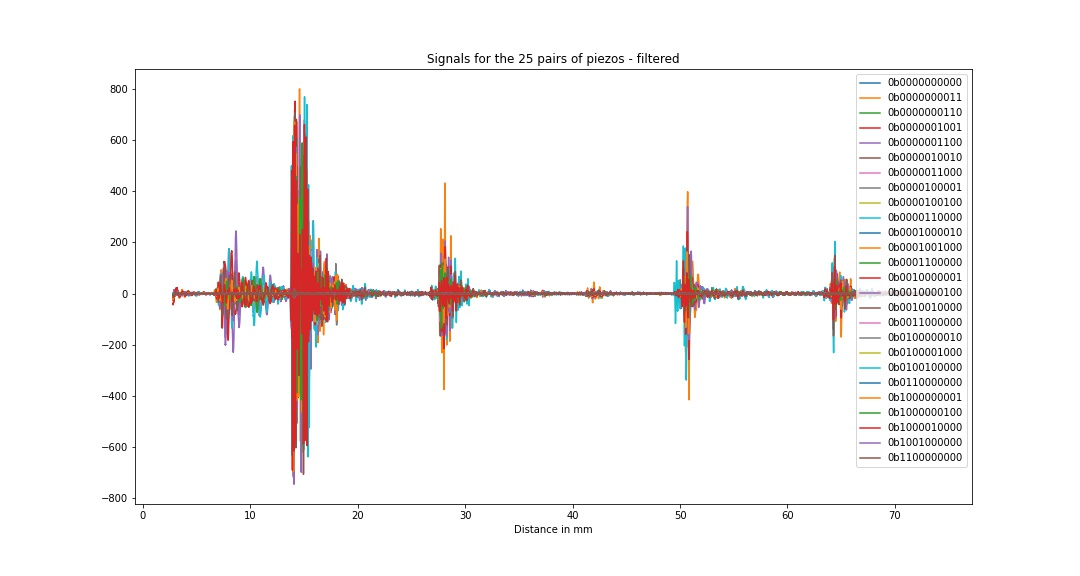
\includegraphics[width=.5\textwidth]{../src/experiment/filtered_sigs.jpg} 
  \caption{Top side of the max14866 board and its connexion to the un0rick.} 
  \label{fig:acq}
\end{figure}



 

\newpage \section{Last details}

\paragraph{Certification}

The development board is open-hardware certified, under ID \href{https://certification.oshwa.org/fr000014.html}{FR000014}.


\paragraph{License}

This work is based on previous projects, the un0rick and the echOmods projects. The lit3rick project and its boards are open hardware and software, developed with open-source elements.

Copyright kelu124 (kelu124@gmail.com) 2020

\begin{itemize}
\item The hardware is licensed under CERN-OHL-S v2.
\item The software components are free software: you can redistribute it and/or modify it under the terms of the GNU General Public License as published by the Free Software Foundation, either version 3 of the License, or (at your option) any later version.
\item The documentation is licensed under a Creative Commons Attribution-ShareAlike 3.0 Unported License.
\end{itemize}


\section{Links to go further}

\begin{itemize}
\item Come and chat : \href{https://join.slack.com/usdevkit/shared_invite/MTkxODU5MjU0NjI1LTE0OTY1ODgxMDEtMmYyZTliZDBlZA}{join the Slack channel} 
\item The full GitHub repository for \href{https://github.com/kelu124/un0rick}{the un0rick "motherboard"}.
\item The board’s \href{https://www.tindie.com/stores/kelu124/}{Tindie shop} to get it
\item The project \href{https://hackaday.io/project/28375-un0rick-an-ice40-ultrasound-board}{ Hackaday page} with more logs
\item Check out \href{https://openhardware.metajnl.com/articles/10.5334/joh.2/}{my previous work} on the topic of ultrasound modules \cite{kelu124} and its \href{http://doi.org/10.5281/zenodo.377054}{dataset on Zenodo}. More to come!

\end{itemize}

 \section{Next steps}

Plenty to do on the next steps! Let me know if you'd like to contribute. The current shopping list (non-exhaustive) may include:

\begin{itemize}
\item Improving the documentation, and updated the work of its \href{https://github.com/kelu124/un0rick}{predecessor, the un0rick} \cite{un0rick}.
\item Shift to a "real", PMOD-compliant connector.
\item Have a better connector
\end{itemize}


\bibliographystyle{unsrt}  
%\bibliography{references}  %%% Remove comment to use the external .bib file (using bibtex).
%%% and comment out the ``thebibliography'' section.


%%% Comment out this section when you \bibliography{references} is enabled.
\begin{thebibliography}{1}

  \bibitem{kelu124}
  Luc Jonveaux 2017.
  \newblock  Arduino-like development kit for single-element ultrasound imaging. 
  \newblock In {\em  Journal of Open Hardware, 1(1), p.3}. DOI: \href{http://doi.org/10.5334/joh.2}{10.5334/joh.2}
  
  \bibitem{un0rick}
  Luc Jonveaux 2019.
  \newblock  un0rick : open-source fpga board for single element ultrasound imaging
  \newblock On {\em  Zenodo}. DOI: \href{http://doi.org/10.5281/zenodo.3364559}{10.5281/zenodo.3364559}
  
  \bibitem{lit3rick}
  Luc Jonveaux 2021.
  \newblock lit3rick: an up5k ultrasound pulse-echo device %%@todo change title
  \newblock On {\em  Zenodo}. DOI: \href{http://doi.org/10.5281/zenodo.5792245}{10.5281/zenodo.5792245}
  
\end{thebibliography}

\end{document}


% Subertley     
%                                             
%  .__  .__  __ ________       .__        __    
%  |  | |__|/  |\_____  \______|__| ____ |  | __
%  |  | |  \   __\_(__  <_  __ \  |/ ___\|  |/ /
%  |  |_|  ||  | /       \  | \/  \  \___|    < 
%  |____/__||__|/______  /__|  |__|\___  >__|_ \
%                      \/              \/     \/
%  